\documentclass[UTF8,a4paper,zihao=-4,fontset=fandol]{ctexart}
% Shared formatting for the course report and research manuscript.
\usepackage[margin=2.2cm,headheight=14pt]{geometry}
\usepackage{amsmath,amssymb,bm,booktabs,tabularx,longtable,array}
\usepackage{graphicx,xcolor,tikz}
\usetikzlibrary{arrows.meta,positioning,calc}
\usepackage{caption,float,placeins}
\usepackage[hidelinks,unicode]{hyperref}
\usepackage{url}
\definecolor{signalblue}{HTML}{205A87}
\definecolor{referenceorange}{HTML}{A95822}
\definecolor{softgray}{HTML}{F0F3F5}
\captionsetup{font=small,labelfont=bf,labelsep=quad}
\renewcommand{\arraystretch}{1.2}
\setlength{\tabcolsep}{4.5pt}
\setlength{\parskip}{0.14em}
\setlength{\emergencystretch}{3em}
\linespread{1.22}
\pagestyle{plain}
\setcounter{tocdepth}{2}
\newcommand{\um}{\,\mu\mathrm{m}}
\newcommand{\ns}{\,\mathrm{ns}}
\newcommand{\mV}{\,\mathrm{mV}}
\newcommand{\fC}{\,\mathrm{fC}}
\newcommand{\V}{\,\mathrm{V}}
\newcommand{\sourcepath}[1]{{\footnotesize\nolinkurl{#1}}}
\graphicspath{{figures/}}
\hypersetup{pdfauthor={},pdfsubject={固定64事件与128响应的r4完整仿真证据；人类课程活动据实待补}}

\newcommand{\EvidenceDate}{2026-10-12 00:34:06 UTC}

\hypersetup{pdftitle={AI辅助下的多特征尺寸DRAM单粒子效应评估：r4完整仿真报告}}
\begin{document}
\begin{titlepage}\centering
\vspace*{1.2cm}
{\zihao{2}\bfseries 项目设计课程报告\par}
\vspace{1.7cm}
{\zihao{1}\bfseries AI辅助下的多特征尺寸DRAM\\[0.35em]单粒子效应评估\par}
\vspace{0.8cm}
{\zihao{3}\color{signalblue}r4完整仿真与验证成果\par}
\vspace{1.5cm}
\begin{tabular}{rl}
指导教师：&李洋（课程大纲所列）\\[1em]
项目成员：&真实姓名、学号与贡献待参与者填写\\[1em]
院系及班级：&待参与者填写\\[1em]
证据快照：&\EvidenceDate
\end{tabular}
\vfill
\begin{minipage}{0.87\textwidth}\small
本报告采用封存并核验的64独立事件、128配对位响应、测试前冻结预测及扩展证据。
工程失败、未知退出码及确定性重试全部保留。技术材料完成不代表学生现场操作、
教师方案审核、试讲、答辩或考核已经发生。模型是未校准二维1T1C探索模型。
\end{minipage}\vspace{1cm}
\end{titlepage}
\pagenumbering{Roman}
\begin{abstract}基于未校准二维平面访问管与理想电容组成的1T1C模型，建立受约束自然语言输入、Geant4电离沉积到TCAD等效源传递、匹配中性参考及测试前预测冻结的评估流程。统一50~$\Omega$预充版本完成四栅长、两粒子、两个方向下64个独立事件和128个0/1配对响应；训练64响应，域内留出与外推各32响应。在5~mV主阈值下，128个响应中96项正确、20项判据误读、8项临界、4项数值不确定，失败和缺失各为0与0项。域内留出的存储0/1岭回归RMSE分别为0.088294/0.094644~fC（电荷）和0.798415/0.838043~mV（裕量损失）。尺寸外推的存储0/1岭回归RMSE分别为0.068049/0.067155~fC（电荷）和0.519434/0.504929~mV（裕量损失）。14项氧化层case与预定两目标的匹配边界细化通过连续门槛，分类跨界和未选近界状态仍保留数值不确定。工程失败、未知退出码与四项确定性重试全部保全，重试和扩展不增加独立事件数。结论限于固定硅入口、二维等效源、受控准静态初态及所选电磁输运配置；不推断持久位翻转、商业DRAM可靠性或辐射截面。
\end{abstract}
\noindent\textbf{关键词：}DRAM；单粒子效应；Geant4；TCAD；匹配参考；冻结预测
\clearpage
{\small\linespread{1.0}\selectfont\tableofcontents}
\clearpage\pagenumbering{arabic}
\ctexset{section={name={第,章},number=\arabic{section}}}
\section{任务目标、基本原理与可行性}
\label{cr:objectives}
\subsection{课程任务与研究对象}
课程要求理解DRAM、单粒子效应和AI基本方法，在个人计算机与远程计算资源之间
搭建仿真环境，完成基础模型、自然语言改参、Geant4到TCAD传递、多参数扫描以及
拟合预测验证，并由2至3名学生合作完成设计、演示和总结\cite{course}。
据此，项目将目标分解为三个可检查的问题：能否把一个明确的粒子条件转换为
可审查的器件源项；能否在相同电学前提下比较不同尺寸和粒子条件的响应；能否
用部分已求解工况预测尚未参与拟合的工况，再由真实TCAD结果检验预测。

本报告选择1T1C DRAM作为对象。一个访问晶体管控制存储节点与位线的连接，
存储电容上的电荷表征信息。保持时访问管关断，读出时字线打开访问管，
存储电容与预充位线发生电荷共享，感测电路据微小差分判别位值\cite{keeth2001}。
因此，“粒子造成多少电荷变化”和“读出是否仍有足够裕量”是相关而不同的问题。
项目既提取保持段电荷扰动，也建立读出指标，避免仅凭存储节点电压下降量判断
完整存储单元的逻辑状态。

\subsection{单粒子效应与数值描述}
载能粒子穿过半导体时产生电子空穴对，载流子在内部电场中漂移，并发生扩散、
复合及端口收集。当扰动到达敏感节点，可能形成瞬态电流或改变储存电荷，
进一步影响电路判读\cite{label1996}。单粒子瞬态、判据上的错误读出与锁存后
持续存在的位翻转并不等价。本项目尚无真实感放锁存和恢复电路，故主要研究
电荷扰动及明确采样时刻的判据裕量。

在漂移扩散框架中，粒子作用以产生率$G$进入电子、空穴连续性方程：
\begin{equation}
\frac{\partial n}{\partial t}=\frac{1}{q}\nabla\!\cdot\mathbf{J}_n+G-R,\qquad
\frac{\partial p}{\partial t}=-\frac{1}{q}\nabla\!\cdot\mathbf{J}_p+G-R.
\end{equation}
这些方程与泊松方程及外部电路方程耦合，决定存储节点和位线的瞬态变化。
Geant4负责粒子输运及能量沉积，TCAD负责沉积之后的半导体电学响应。
二者之间的接口必须明确材料、坐标、单位、源项形状及有效厚度；工具同时运行
并不足以证明它们描述了相同的物理对象。

\subsection{可行性与实际设计过程}
实际环境由Windows本机承担请求解析、批次管理、归档和后处理，由已有Linux
虚拟机运行Geant4与Sentaurus。本机通过严格SSH入口访问虚拟机，保留命令、
返回状态和输入输出摘要。这实现了远程访问式工作流，但现有材料没有提供
实验室独立服务器或正式资源交接记录，不能把虚拟机使用记录替代课程要求中的
资源交接。现有软件、许可证和脚本已能支持单核串行求解，主要成本来自TCAD
瞬态和必要复验，而非表格或绘图。

设计采用逐级建立证据的方式。v1先用小矩阵贯通真实输运、器件响应与外推；
v2加入统一初态、0/1配对和读出判据；D1进一步追查理想参考留下的读出偏移；
随后R50-main以匹配中性参考及统一预充版本建立更完整的矩阵。
这种过程让前一阶段暴露的问题成为后一阶段的设计依据。
当前报告以共享证据快照为截止点，完成状态见表\ref{cr:progress}；
历史阶段保留其原条件，不用新模型重写旧结论\cite{project}。

\section{基础模型与参数来源}
\label{cr:model}
\subsection{几何、电路与物理假设}
基础模型为自编二维平面NMOS加理想存储电容的1T1C单元。设栅长为$L$，
硅体宽度为$L+0.6\um$、深度为$1.2\um$，二维有效第三维厚度为$1\um$。
主模型氧化层厚度为$5\,\mathrm{nm}$，体区为P型，体掺杂浓度
$10^{17}\,\mathrm{cm}^{-3}$，源漏高斯峰值为$10^{20}\,\mathrm{cm}^{-3}$，
结深参数为$0.12\um$。栅功函数设为$4.6\,\mathrm{eV}$，
温度为$300\,\mathrm{K}$，外接存储电容为$10\,\mathrm{fF}$。
比较的四个栅长是$0.18/0.25/0.35/0.45\um$，表示访问晶体管的几何长度，
并不表示商业DRAM工艺节点。

模型使用Fermi统计、OldSlotboom带隙修正、掺杂和电场相关迁移率以及
SRH、Auger复合。器件采用漂移扩散求解，电路节点同时参与瞬态计算。
选用这种结构的依据是它保留了访问管、电荷存储及电荷共享三项基本机制，
输入规模适合当前计算环境，也便于检查粒子源与电路响应之间的关系。
真实DRAM可能采用复杂沟道、埋栅和立体电容，简化结构不能替代这些工艺的
电学标定，更不能由栅长数值推断产品代际。

\begin{table}[htbp]
\centering\small
\caption{主模型参数与证据性质。数值为本项目冻结的探索参数，不能统一称为文献实测值。}
\label{cr:parameters}
\begin{tabularx}{\textwidth}{lllX}
\toprule
参数&主模型取值&用途&来源或适用范围\\
\midrule
栅长$L$&0.18至0.45 $\mu$m&几何扫描&自编平面访问管，四点离散取值\\
氧化层&5 nm&主矩阵&4/6 nm为独立受控变体，结果见第5章\\
存储电容&10 fF&储存电荷&1T1C原理与已有混合模式示例支持形式，未校准器件\\
位线与参考电容&100 fF&读出电荷共享&统一电路假设，便于匹配比较\\
初态SN&0.1/0.9 V&存储0/1&理想钳位与准静态初态，非写入校准\\
中性参考SN&0.5 V&消除共模偏移&同器件、同网格与时序的参考支路\\
预充导通电阻&50 $\Omega$&R50-main读出&由独立probe支持的物理修订\\
\bottomrule
\end{tabularx}
\end{table}

\subsection{从参数来源到可检验假设}
参数来源分为原理、工具约定、已有模型形式和本项目假设四类。
DRAM教材支持访问晶体管与电容的基本工作机制；Geant4资料支持输运过程和
电磁模型的含义\cite{keeth2001,g4em}。已有混合模式DRAM示例说明外接理想
电容的建模方式可行，但本项目没有复制并校准其完整工艺工程。
几何尺寸、掺杂、位线电容及裕量门槛仍按探索假设处理。用明确的来源分层，
可以把“软件支持这个模型”与“模型代表某种真实器件”区分开来。

R50-main的0/1状态通过理想SN钳位获得，钳位在$0.6\ns$释放，
并在$0.95\ns$检查初态误差不超过$1\mV$。这一设置减少不同栅长写入程度
不同所带来的混杂，使比较更接近“相同初态下的访问管几何变化”。
然而它只控制初始电压，不证明实际写入时间、能耗或访问管写入能力。
v1曾采用实际访问管充电，不同栅长的粒子前电压不同；
因此两版数据适合解释设计改进，不能拼接成一条统一的尺寸响应曲线。

\subsection{保持、预充与匹配参考}
粒子在$1\ns$注入，保持指标在$2.8\ns$提取。位线随后经预充支路升至
$0.5\V$，在$3\ns$释放；字线在$3.05$至$3.10\ns$升至$1.8\V$，
读出在$4\ns$采样。R50-main使用$50\,\Omega$导通电阻，
关断电阻为$10^{20}\,\Omega$，不把理想开关的电压跳变当作预充完成。

匹配中性参考在相同尺寸、网格、偏压及时序下取SN=$0.5\V$。
批量计算使用信号位线与中性参考位线之差，并先通过真实双支路仿真核对。
这种参考随访问管打开而产生相应的耦合和电荷交换，比统一减去一个常数更适合
处理状态相关偏移。参考中不注入粒子；物理双支路中采用独立器件定义，
以防同一HeavyIon设置同时作用于信号与参考。

\section{AI交互平台与Geant4到TCAD的传递}
\label{cr:platform}
\subsection{自然语言、结构化设计与执行边界}
AI在项目中辅助阅读文献、组织假设、生成和检查脚本、定位失败、提取结果及
撰写解释。可以被复验的交互接口则是限定中文模板：请求明确列出栅长、
粒子、能量、方向、重复数和范围，解析后得到结构化工况清单。
每个工况包含几何条件、粒子条件、种子、配对位值及训练或测试身份。
接口拒绝模糊尺寸、未支持角度和超出冻结范围的要求，避免把自然语言中的
省略或歧义直接传给求解器。

v1已有中文请求生成完整矩阵并进入真实执行链路的记录。
当前R50演示入口提供\texttt{preview}、\texttt{audit}和\texttt{locate}：
分别预览映射、检查接受与拒绝行为、定位指定事件的证据路径。
它只说明请求与已冻结R50设计如何对应，不自动提交新求解。
$50\,\Omega$来自版本化物理修订，而非解析器从句子中猜测出的参数。
自然语言成功解析是软件层的检查，实际模型正确性仍由后续物理与数值证据判定。

\begin{figure}[htbp]
\centering
% Conceptual workflow, not a measured result or screenshot.
\resizebox{\linewidth}{!}{%
\begin{tikzpicture}[
 block/.style={draw=signalblue,rounded corners=2pt,fill=softgray,
 text width=4.2cm,minimum height=1.5cm,align=center,font=\small},
 arrow/.style={-{Latex[length=2.4mm]},thick,draw=signalblue},
 node distance=0.7cm and 0.6cm]
\node[block] (request) {限定中文请求\\尺寸、粒子、角度\\独立事件数};
\node[block,right=of request] (matrix) {受约束的工况清单\\单位、范围、版本与种子};
\node[block,right=of matrix] (transport) {Geant4 硅内电离沉积\\$E_{\rm ion}\ \rightarrow\ Q_{\rm dep}$\\有限径迹及单位检查};
\node[block,below=of transport] (tcad) {TCAD 器件与电路求解\\等效径迹与受控初态\\读出瞬态与端口检查};
\node[block,left=of tcad] (metric) {匹配中性参考与同位对照\\$D,\ M,\ \Delta Q,\ \Delta M$};
\node[block,left=of metric] (model) {按工况分组的响应拟合\\冻结预测后检验未见响应};
\draw[arrow] (request)--(matrix);
\draw[arrow] (matrix)--(transport);
\draw[arrow] (transport)--(tcad);
\draw[arrow] (tcad)--(metric);
\draw[arrow] (metric)--(model);
\node[below=0.40cm of metric,align=center,font=\small,text width=14.5cm]
 {每一层绑定输入版本、运行记录和来源哈希；科学质量门槛与执行状态分别记录。};
\end{tikzpicture}}

\caption{AI辅助联合评估的工作流程示意。自然语言请求经结构化审查与冻结后，
连接粒子输运、等效源传递、器件求解和独立评价；此图为流程示意，不代表未完成阶段已有结果。}
\label{cr:workflow}
\end{figure}

\subsection{输运记录与等效源转换}
Geant4在硅与真空组成的简化几何中运行电磁option4及步长限制，
记录每一步的位置、时间、总沉积能、非电离沉积能和轨迹身份。
主矩阵采用$5\,\mathrm{MeV}$的$\alpha$粒子与质子，方向为0°和30°，
表面入射位置与各栅长模型保持约定关系。30°径迹可能从侧面退出，
因此不能机械地把硅深度除以角度余弦视为所有工况的有效径迹长度。
实际几何交点及源文件共同决定传递参数。

只把硅内电离能量计入电子空穴对产生。设逐步电离沉积总量为
$E_{\mathrm{ion}}$，使用硅中平均$3.6\,\mathrm{eV}$产生一对载流子的近似，
得到
\begin{equation}
N_{\mathrm{eh}}=\frac{10^6E_{\mathrm{ion}}[\mathrm{MeV}]}{3.6},\qquad
Q_{\mathrm{dep}}=qN_{\mathrm{eh}},\qquad
\mathrm{LET}_{\mathrm{eq}}=\frac{Q_{\mathrm{dep}}}{\ell}.
\label{cr:transfer}
\end{equation}
式中$\ell$是约定的硅内等效直径迹长度。TCAD以半径$0.03\um$的
Gaussian HeavyIon源注入等效电荷，并使用一致的二维有效厚度和电荷单位。
这一方法保留事件的电离总量，便于小规模参数扫描；逐步输运CSV仍单独保留，
以便识别总量近似忽略的纵向、横向和时间分布信息。

已有TCAD与Geant4的SRAM评估研究提供了联合方法的先例\cite{chen2011}；
硅二极管中重离子、聚焦X射线和脉冲激光的瞬态比较，则提示不同电荷产生方式
需要分别处理\cite{ryder2021}。这些文献不能直接校准本项目的DRAM模型。
本项目采用总量等效直径迹而非完整三维产生率网格，
故需要分别检查转换算术与TCAD实际源积分。前者核对单位和总电荷，
后者检查离散网格、径迹截断和时间积分之后是否仍近似注入目标电荷。
二者通过并不意味着空间分布误差消失。

\subsection{可追溯执行与数据流}
执行流程将设计、输入deck、Geant4事件三文件、求解日志及输出归档绑定到唯一
run ID，并用SHA-256检查内容一致性。续算只允许使用同几何、同电路、同网格和
已核对合同的保存点；改变网格或参考结构后重新建立相应初态。
主运行器负责归档，分析器从固定原始输出提取曲线，图表再引用这些曲线和摘要，
形成“请求—输入—源—求解—指标—图”的连续来源关系。

这种设计尤其适合AI辅助操作。AI能够快速生成大量命令，也可能误读旧摘要、
把同名文件当作同一内容，或把后台退出当成远端求解停止。
因此流程把可机器检查的版本与完成条件写入入口，而不是依赖对话记忆。
报告中的数据图属于原始数值后处理；真实Sentaurus窗口截图和原生场图另行标注，
防止用美观的曲线图替代软件求解证据。

\section{实验矩阵、预测设计与验证方法}
\label{cr:design}
\subsection{固定矩阵与响应定义}
R50-main主设计包含四种栅长、两种粒子和两个方向，每个组合预定四个独立种子，
共64个独立粒子事件；每个事件分别施加于存储0和存储1，形成128个响应槽位。
配对设计有助于识别位值不对称，但同一沉积事件的两种初态不构成两个独立入射。
数值复跑、网格细化、参考诊断和氧化层配对同样不增加独立事件数。
所有种子与工况在读取正式响应前登记，失败不通过更换种子补成有利样本。

R50-main使用如下连续指标：
\begin{align}
\Delta Q&=C_{\mathrm{store}}\,[V_{\mathrm{SN,event}}(2.8\ns)
 -V_{\mathrm{SN,control}}(2.8\ns)],\\
D(t)&=V_{\mathrm{BL,signal}}(t)-V_{\mathrm{BL,neutral}}(t),\\
M&=(2b-1)D(4\ns),\qquad
\Delta M=M_{\mathrm{control}}-M_{\mathrm{event}}.
\label{cr:metrics}
\end{align}
其中control是同位值无粒子对照，neutral是中性参考，两者功能不同。
$\Delta Q$保留符号，负值表示事件SN低于对照；$\Delta M>0$表示裕量退化。
对存储0而言，节点进一步下降可能使判据裕量增加，此时$\Delta M$可以为负，
不应把所有变化都强制写成非负的“损伤”。

主判据取$\varepsilon=5\mV$：$M>\varepsilon$为正确，
$M<-\varepsilon$为判据误读，其余为临界。
同时保留$2.5/10\mV$阈值结果。接近边界而未完成规定数值复验、
或粗细离散分类不一致时，另列数值不确定；失败和缺失保持各自状态。
统计按冻结分母报告，不用可判子集替代预定样本。

\subsection{分组拟合与测试前冻结}
训练集取$L=0.18/0.35\um$，共32个事件、64个响应；
$0.25\um$为域内留出，$0.45\um$为尺寸外推，各16个事件、32个响应。
同一物理事件及其配对结果保持同组，避免相同源信息同时出现在训练和测试中。
预测使用真实Geant4沉积量，目标是在给定沉积与无粒子条件下近似TCAD响应。
它有望减少后续器件求解成本，但仍须获得粒子输运输入。

分别针对两种位值的$\Delta Q$与$\Delta M$建立四个岭回归模型，
特征为$Q_{\mathrm{dep}}$、$Q_{\mathrm{dep}}/L$和
$Q_{\mathrm{dep}}\sin\theta$。这些项以电荷注入规模、尺寸及方向为物理启发，
并不是已推导出的通用器件定律。与训练均值基准比较，可检查回归是否比
忽略输入变量更有信息；数据驱动单粒子响应建模的相关研究也为这种代理思路
提供背景\cite{xu2021}。

训练采用留一物理工况交叉验证（LOCO）。训练区有八个尺寸、粒子、角度组合，
每折将一个完整组合的四个重复留出；两位保持相同的分组边界。
标准化均值和方差只由本折训练数据计算。候选正则化参数为
$0,0.01,0.1,1,10$，以八折RMSE的算术均值选择，不由测试集选模。
岭目标为
\begin{equation}
\min_{\beta_0,\boldsymbol\beta}
\sum_i(y_i-\beta_0-\boldsymbol z_i^{\mathsf T}\boldsymbol\beta)^2
+\lambda\|\boldsymbol\beta\|_2^2,
\end{equation}
截距不惩罚。最终参数用完整训练集拟合，在首次测试TCAD提交前冻结模型、
标准化参数、Geant4测试输入、64条逐位预测及其哈希。
留出和外推完成后仅计算误差，不再按测试误差修改模型。

\subsection{分层验证与工程验收}
每个有效响应需满足完整求解到$4\ns$、有限数据、初态误差不超过$1\mV$、
预充误差不超过$10\,\mu\mathrm{V}$，并检查逐相KCL、四端口闭合和
后向欧拉右端点电荷积分。粒子源实际积分与目标Q的偏差门槛为5\%，
参考支路源项应为零。对物理双支路和离线参考同时比较两侧BL及差分，
防止两侧误差偶然抵消。

预登记代表点分别进行半时间步和0.7网格尺度检查，并为每个变体匹配自己的
对照和中性参考。$\Delta M$变化门槛为$0.5\mV$、$\Delta Q$为$0.01\fC$，
同时核对分类稳定性。训练交叉验证、数值细化和独立测试解决不同问题：
前者检验训练工况内的拟合选择，中者检查离散敏感性，后者检验未见尺寸条件。
任何一项通过都不能自动替代另外两项。

\section{全量响应、预测与扩展结果}
\label{cr:results}
\subsection{封存快照与样本完成度}
本次证据截止为\EvidenceDate。完整训练和测试均经原档重审，未读取在途或原FAILED电学输出。四alias仅提供其原逻辑槽，来源含实际run、owner plan、case-freeze与输入/归档SHA。
快照内部分图件状态保留采集时的PENDING标签，未回写历史快照；后续完整机器、统计和逐图目视验收另见\sourcepath{data/delivery-root-acceptance.json}及两份visual-review记录。本文将采集时状态与事后验收证书分开引用。

\begin{table}[htbp]
\centering\small
\caption{完整主矩阵的样本与响应分配；同事件两位不独立翻倍。}
\label{cr:progress}
\begin{tabular}{lrrrr}
\toprule
集合 & 独立事件 & 配对响应 & 已验证 & 缺失\\
\midrule
训练0.18/0.35 $\mu$m & 32 & 64 & 64 & 0\\
域内0.25 $\mu$m & 16 & 32 & 32 & 0\\
外推0.45 $\mu$m & 16 & 32 & 32 & 0\\
\bottomrule
\end{tabular}

\end{table}
\subsection{匹配参考与预充修订的历史依据}
历史D1无粒子诊断中，固定理想参考留下约12.37~mV读出偏移；同一信号状态改用匹配中性参考后，差分从+2.454961~mV变为-9.915036~mV。该诊断说明参考会改变判据解释，不纳入R50主矩阵。原100~$\Omega$固定事件的3~ns预充误差为-13.297362~$\mu$V，超过10~$\mu$V原门槛；独立50~$\Omega$ probe对应误差为-4.731204~$\mu$V，随后才建立独立统一主版本。

\begin{figure}[htbp]
\centering
\includegraphics[width=.85\textwidth]{d1-reference-comparison.pdf}
\caption{历史D1参考诊断，仅用于解释方法演进；原始分类不追溯替换。}
\label{cr:d1}
\end{figure}

\begin{figure}[htbp]
\centering
\includegraphics[width=.85\textwidth]{r50-precharge.pdf}
\caption{历史100~$\Omega$失败与独立50~$\Omega$ probe。两者均不作为新的R50主事件。}
\label{cr:precharge}
\end{figure}
\subsection{完整128响应与三阈值统计}
在5~mV主阈值下，128个响应中96项正确、20项判据误读、8项临界、4项数值不确定，失败和缺失各为0与0项。
每个尺寸/粒子/方向/位值分层的预定N保持4，零次明确误读不能推出总体风险为零。表中有效分类已传播近界和细化跨界不确定性，原分类另见完整响应CSV。

\begin{table}[htbp]
\centering\small
\caption{完整128响应在三阈值下的有效状态；失败与缺失不计为正确。}
\label{cr:thresholds}
\begin{tabular}{rrrrrrr}
\toprule
阈值/mV & 正确 & 判据误读 & 临界 & 数值不确定 & 失败 & 缺失\\
\midrule
2.5 & 96 & 27 & 4 & 1 & 0 & 0\\
5 & 96 & 20 & 8 & 4 & 0 & 0\\
10 & 96 & 5 & 26 & 1 & 0 & 0\\
\bottomrule
\end{tabular}

\end{table}

\begin{table}[htbp]
\centering\footnotesize
\caption{按栅长、粒子、位值列出的连续响应范围；每行合并两方向共8响应，未额外增加独立样本。}
\label{cr:ranges}
\begin{tabular}{lclrrr}
\toprule
$L$/\,$\mu$m & 粒子 & 位 & $\Delta Q$/fC & $\Delta M$/mV & $M$/mV\\
\midrule
0.18 & $\alpha$ & 0 & -4.821至-3.560 & -45.514至-33.619 & 71.116至83.011\\
0.18 & $\alpha$ & 1 & -5.412至-3.967 & 37.026至50.550 & -13.213至0.311\\
0.18 & 质子 & 0 & -0.402至-0.164 & -3.784至-1.545 & 39.041至41.281\\
0.18 & 质子 & 1 & -0.436至-0.181 & 1.685至4.066 & 33.270至35.651\\
0.25 & $\alpha$ & 0 & -4.701至-3.732 & -44.357至-35.148 & 72.537至81.746\\
0.25 & $\alpha$ & 1 & -5.166至-4.118 & 38.339至48.114 & -10.880至-1.105\\
0.25 & 质子 & 0 & -0.460至-0.239 & -4.317至-2.241 & 39.631至41.706\\
0.25 & 质子 & 1 & -0.496至-0.257 & 2.391至4.609 & 32.626至34.844\\
0.35 & $\alpha$ & 0 & -4.862至-4.081 & -45.601至-38.220 & 75.376至82.757\\
0.35 & $\alpha$ & 1 & -5.307至-4.459 & 41.259至49.125 & -12.119至-4.253\\
0.35 & 质子 & 0 & -0.456至-0.145 & -4.250至-1.354 & 38.510至41.406\\
0.35 & 质子 & 1 & -0.488至-0.155 & 1.435至4.509 & 32.496至35.571\\
0.45 & $\alpha$ & 0 & -4.834至-3.886 & -45.066至-36.161 & 73.090至81.994\\
0.45 & $\alpha$ & 1 & -5.249至-4.208 & 38.699至48.287 & -11.506至-1.918\\
0.45 & 质子 & 0 & -0.509至-0.229 & -4.716至-2.120 & 39.048至41.645\\
0.45 & 质子 & 1 & -0.544至-0.244 & 2.237至5.000 & 31.781至34.544\\
\bottomrule
\end{tabular}

\end{table}

\begin{figure}[htbp]
\centering
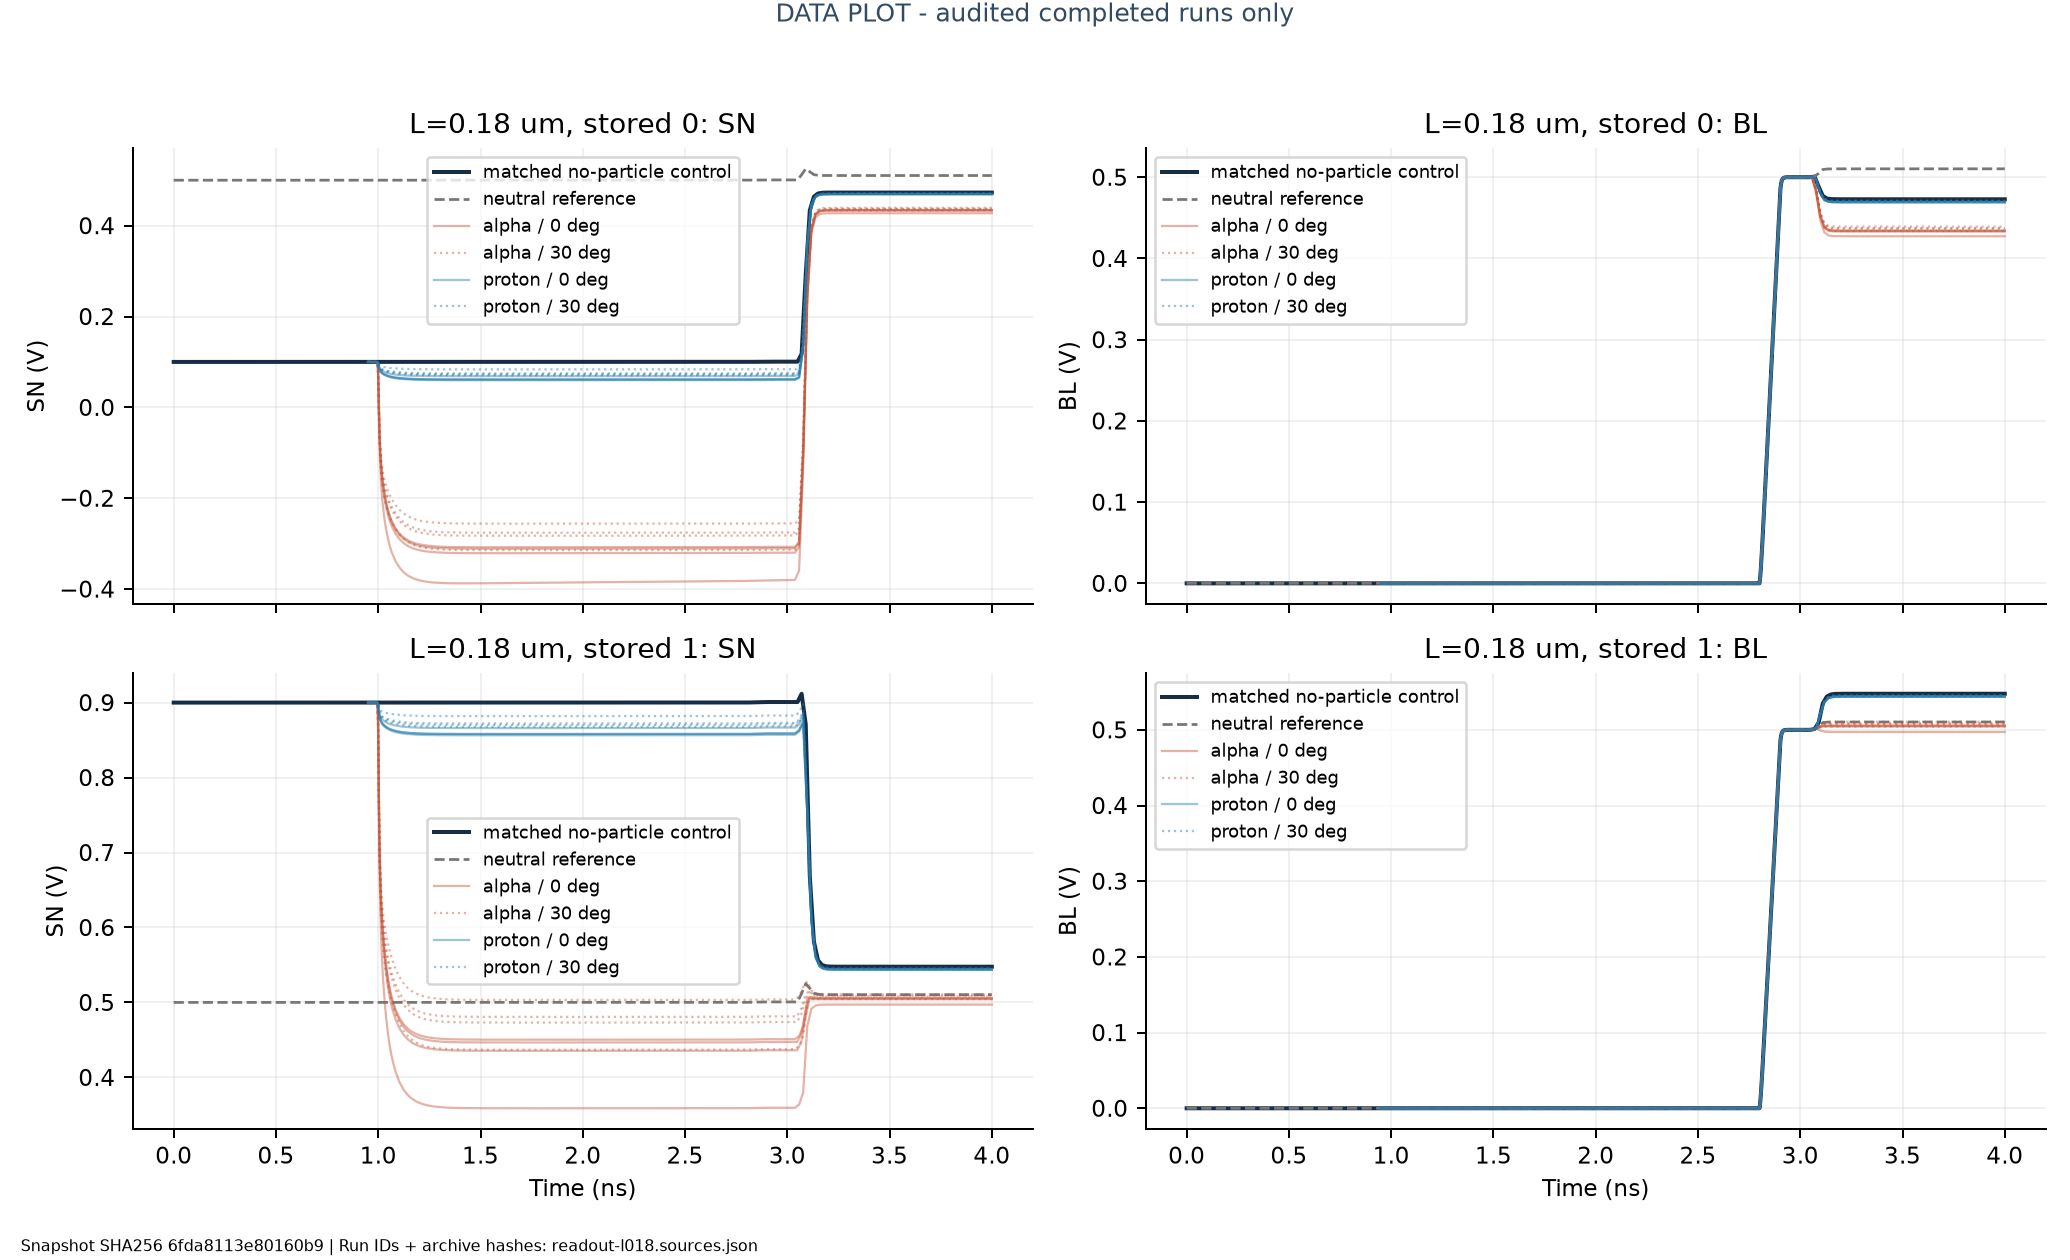
\includegraphics[width=.95\textwidth]{readout-l018.png}
\caption{0.18~$\mu$m的全部事件、同位control与neutral读出曲线；数据来自统一R50快照。}
\label{cr:readout}
\end{figure}

\begin{figure}[htbp]
\centering
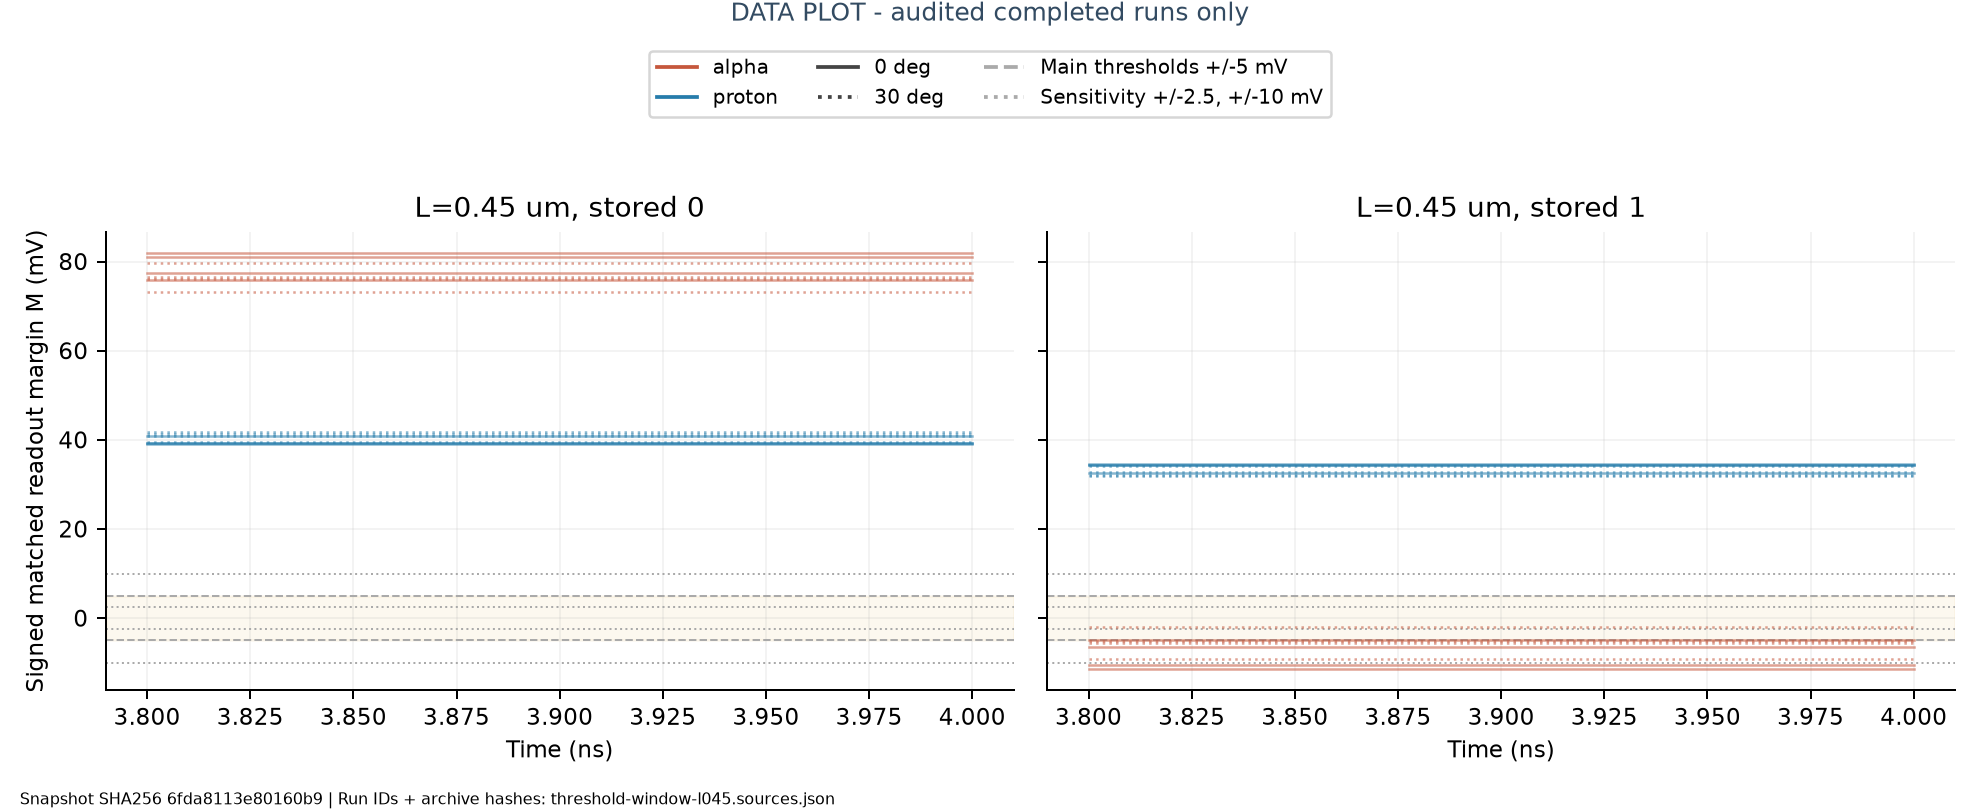
\includegraphics[width=.95\textwidth]{threshold-window-l045.png}
\caption{0.45~$\mu$m外推集合在3.8至4~ns的读出裕量窗口；线条和阈值均来自封存快照。}
\label{cr:window}
\end{figure}
\subsection{原冻结模型的独立留出与外推}
四模型由训练工况LOCO选择，冻结后不再调参。
\begin{table}[htbp]
\centering\small
\caption{八个物理工况折RMSE的算术平均；仅用于训练阶段模型选择。}
\label{cr:cv}
\begin{tabular}{llrrr}
\toprule
位 & 目标 & $\lambda$ & 岭回归RMSE & 均值基准RMSE\\
\midrule
0 & $\Delta Q$/fC & 0.1 & 0.102888 & 2.279967\\
0 & $\Delta M$/mV & 0.1 & 0.955160 & 21.458870\\
1 & $\Delta Q$/fC & 0.1 & 0.112903 & 2.515710\\
1 & $\Delta M$/mV & 0.1 & 1.012491 & 23.383861\\
\bottomrule
\end{tabular}

\end{table}
域内留出的存储0/1岭回归RMSE分别为0.088294/0.094644~fC（电荷）和0.798415/0.838043~mV（裕量损失）。尺寸外推的存储0/1岭回归RMSE分别为0.068049/0.067155~fC（电荷）和0.519434/0.504929~mV（裕量损失）。本次原r4评分与最终连续有效性评分逐项一致。
分类临界或跨界与连续量有效性分别处理；原r4首次评分的原字节副本与最终数值评分均附在证据包。

\begin{table}[htbp]
\centering\footnotesize
\caption{$\Delta Q$的固定预测误差，单位fC。每模型/位/集合计划16响应；缺失和无效显式报告。}
\label{cr:scoreq}
\begin{tabular}{lllrrrrrr}
\toprule
集合 & 位 & 模型 & $n$ & 缺失 & 无效 & MAE & RMSE & 最大误差\\
\midrule
留出 & 0 & 均值基准 & 16 & 0 & 0 & 1.942616 & 1.956036 & 2.416036\\
留出 & 0 & 岭回归 & 16 & 0 & 0 & 0.056607 & 0.088294 & 0.181592\\
留出 & 1 & 均值基准 & 16 & 0 & 0 & 2.140865 & 2.154850 & 2.651122\\
留出 & 1 & 岭回归 & 16 & 0 & 0 & 0.061766 & 0.094644 & 0.198945\\
外推 & 0 & 均值基准 & 16 & 0 & 0 & 2.011262 & 2.025386 & 2.548969\\
外推 & 0 & 岭回归 & 16 & 0 & 0 & 0.052826 & 0.068049 & 0.136393\\
外推 & 1 & 均值基准 & 16 & 0 & 0 & 2.183932 & 2.198297 & 2.733561\\
外推 & 1 & 岭回归 & 16 & 0 & 0 & 0.051740 & 0.067155 & 0.144228\\
\bottomrule
\end{tabular}

\end{table}

\begin{table}[htbp]
\centering\footnotesize
\caption{$\Delta M$的固定预测误差，单位mV。测试没有反向参与选模。}
\label{cr:scorem}
\begin{tabular}{lllrrrrrr}
\toprule
集合 & 位 & 模型 & $n$ & 缺失 & 无效 & MAE & RMSE & 最大误差\\
\midrule
留出 & 0 & 均值基准 & 16 & 0 & 0 & 18.320612 & 18.448022 & 22.860163\\
留出 & 0 & 岭回归 & 16 & 0 & 0 & 0.526964 & 0.798415 & 1.645649\\
留出 & 1 & 均值基准 & 16 & 0 & 0 & 19.936695 & 20.066626 & 24.741705\\
留出 & 1 & 岭回归 & 16 & 0 & 0 & 0.549768 & 0.838043 & 1.765441\\
外推 & 0 & 均值基准 & 16 & 0 & 0 & 18.742144 & 18.867683 & 23.569637\\
外推 & 0 & 岭回归 & 16 & 0 & 0 & 0.404964 & 0.519434 & 1.075289\\
外推 & 1 & 均值基准 & 16 & 0 & 0 & 20.091257 & 20.219896 & 24.915029\\
外推 & 1 & 岭回归 & 16 & 0 & 0 & 0.387723 & 0.504929 & 1.105078\\
\bottomrule
\end{tabular}

\end{table}

\begin{figure}[htbp]
\centering
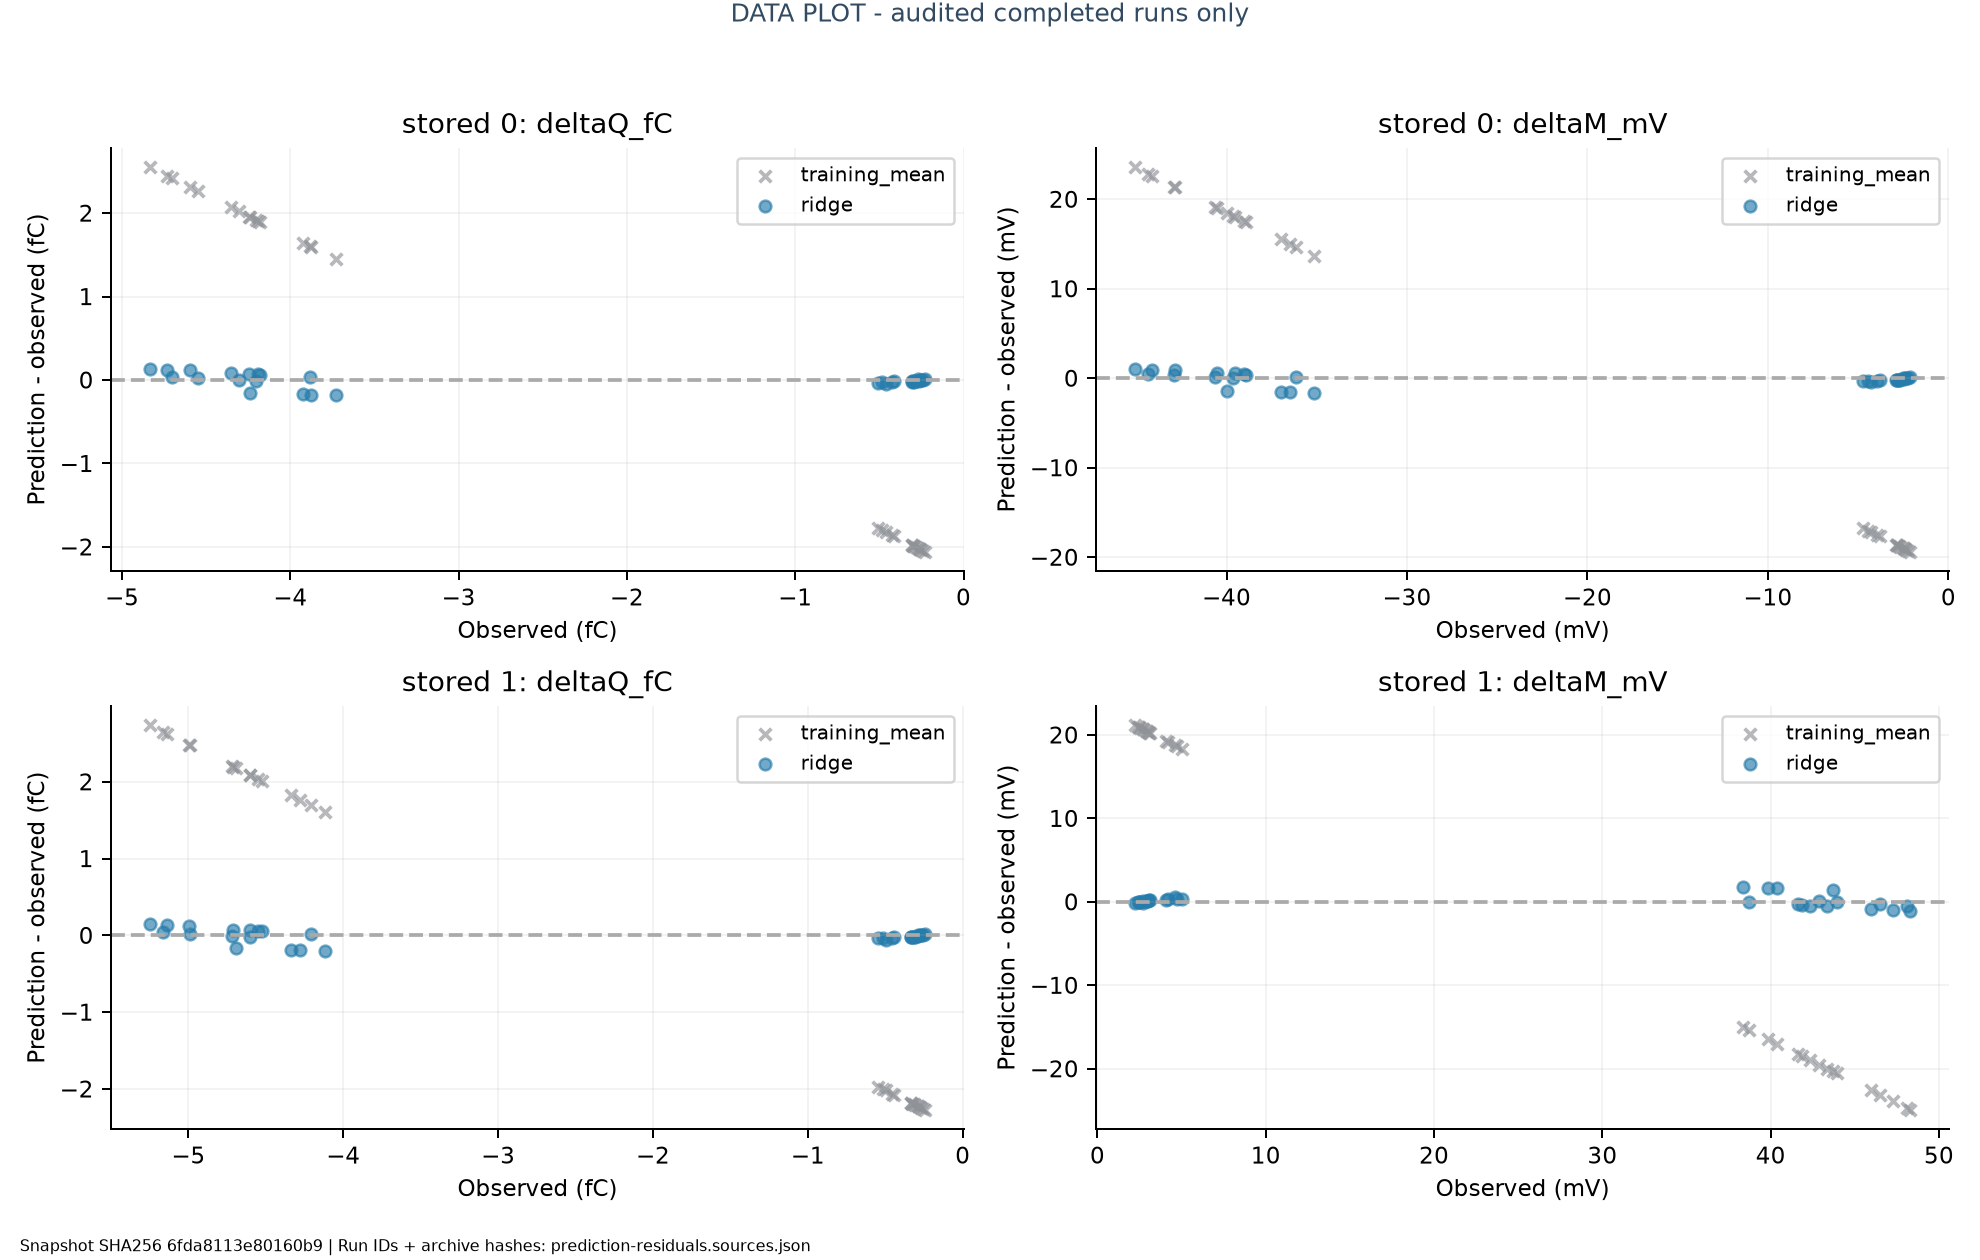
\includegraphics[width=.95\textwidth]{prediction-residuals.png}
\caption{冻结预测减去实际观测的留出/外推残差；训练均值与岭回归均保留。}
\label{cr:residuals}
\end{figure}
\subsection{氧化层敏感性}
在0.25~$\mu$m、垂直入射的固定alpha/质子首个事件上，4/6~nm厚度各建立独立0/1对照、中性参考和事件响应，共14个case。5~nm复用对应四个主响应；含原质子bit0的r3有效alias。每个新厚度实际重建网格，事件三文件字节保持一致。

\begin{table}[htbp]
\centering\footnotesize
\caption{相对于对应5~nm响应的氧化层变化；$\delta(\Delta Q)$和$\delta(\Delta M)$是新厚度减5~nm。}
\label{cr:oxide}
\begin{tabular}{llrrrr}
\toprule
粒子 & 位 & $t_{ox}$/nm & $\delta(\Delta Q)$/fC & $\delta(\Delta M)$/mV & $M$/mV\\
\midrule
$\alpha$ & 0 & 4 & -0.00240 & 0.06772 & 77.8443\\
$\alpha$ & 0 & 6 & -0.00578 & -0.11012 & 78.1679\\
$\alpha$ & 1 & 4 & -0.00464 & -0.06297 & -6.7275\\
$\alpha$ & 1 & 6 & -0.00484 & 0.11256 & -6.7559\\
质子 & 0 & 4 & -0.00022 & 0.00324 & 39.5380\\
质子 & 0 & 6 & -0.00028 & -0.00589 & 39.6928\\
质子 & 1 & 4 & -0.00022 & -0.00377 & 34.7574\\
质子 & 1 & 6 & -0.00027 & 0.00621 & 34.8945\\
\bottomrule
\end{tabular}

\end{table}

\begin{figure}[htbp]
\centering
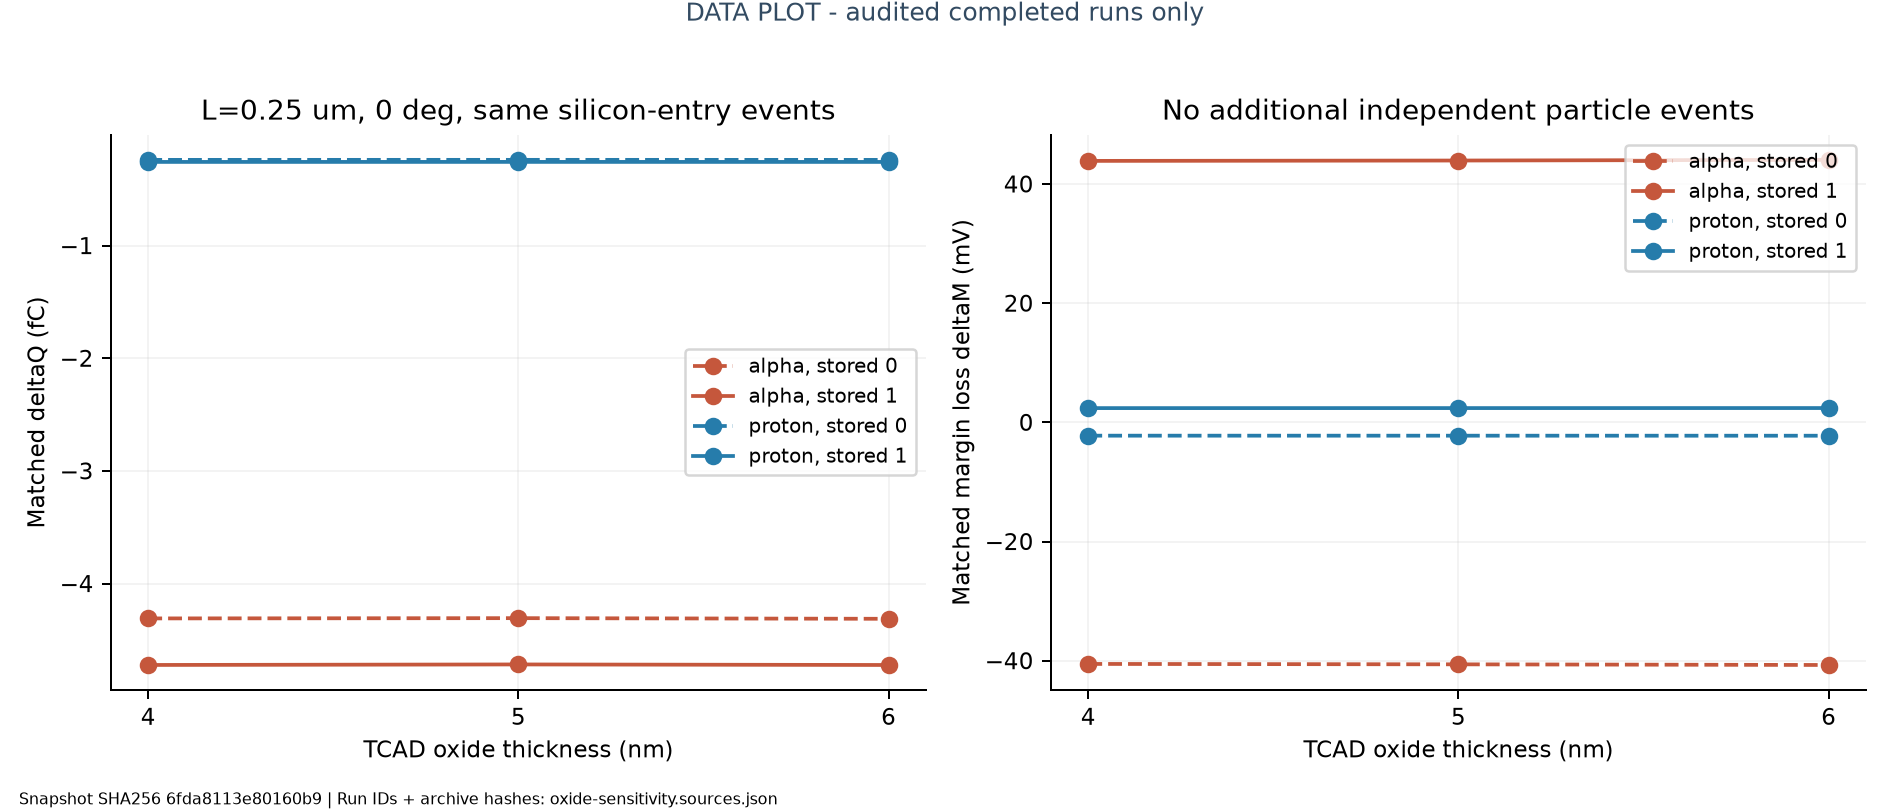
\includegraphics[width=.95\textwidth]{oxide-sensitivity.png}
\caption{4/5/6~nm在固定硅入口事件下的TCAD敏感性；不表示变化材料栈的Geant4输运。}
\label{cr:oxidefig}
\end{figure}
八个新事件响应相对于5~nm的最大绝对变化为0.112560497~mV（裕量损失）和约0.005783687~fC（电荷），分类保持。这些幅度小于预定验收容差0.5~mV和0.01~fC；容差不是统计误差条或已估计的分辨率。每个氧化层响应未再做独立细化和统计校准，故只报告固定入口事件下幅度较小的受控敏感性，不主张零效应、微小效应已可靠分辨或统计显著性。
\subsection{完整矩阵边界细化与原生图}
边界目标由完整128响应到$\pm2.5/5/10$~mV的最小距离排序选取，保持原规则和目标。每目标分别使用半步长与0.7网格的匹配control/neutral/event。四项连续比较均通过，但连续通过不代表类别稳定；5~mV跨界及未选近界响应继续保留不确定性。

\begin{table}[htbp]
\centering\footnotesize
\caption{四个边界比较。最大电压变化包含规定的两侧BL与派生读出量；容差0.5~mV和0.01~fC。}
\label{cr:boundary}
\begin{tabular}{llrrll}
\toprule
事件/位 & 变体 & 最大电压变化/mV & $|\delta\Delta Q|$/fC & 连续门槛 & 不确阈值/mV\\
\midrule
202610304/b1 & 半步长 & 0.032654 & 0.003490 & 通过 & 5\\
202610304/b1 & 0.7网格 & 0.005088 & 0.000009 & 通过 & 无\\
202610313/b1 & 半步长 & 0.025337 & 0.002709 & 通过 & 无\\
202610313/b1 & 0.7网格 & 0.005088 & 0.000006 & 通过 & 无\\
\bottomrule
\end{tabular}

\end{table}

\begin{table}[htbp]
\centering\small
\caption{128响应乘三阈值的384个状态。界外未细化不冒称全部网格独立。}
\label{cr:uncertainty}
\begin{tabular}{lr}
\toprule
阈值响应对状态 & 数量/384\\
\midrule
细化稳定 & 8\\
分类跨界 & 1\\
连续失败 & 0\\
近界待确认 & 5\\
界外未细化 & 370\\
\bottomrule
\end{tabular}

\end{table}

\begin{figure}[htbp]
\centering
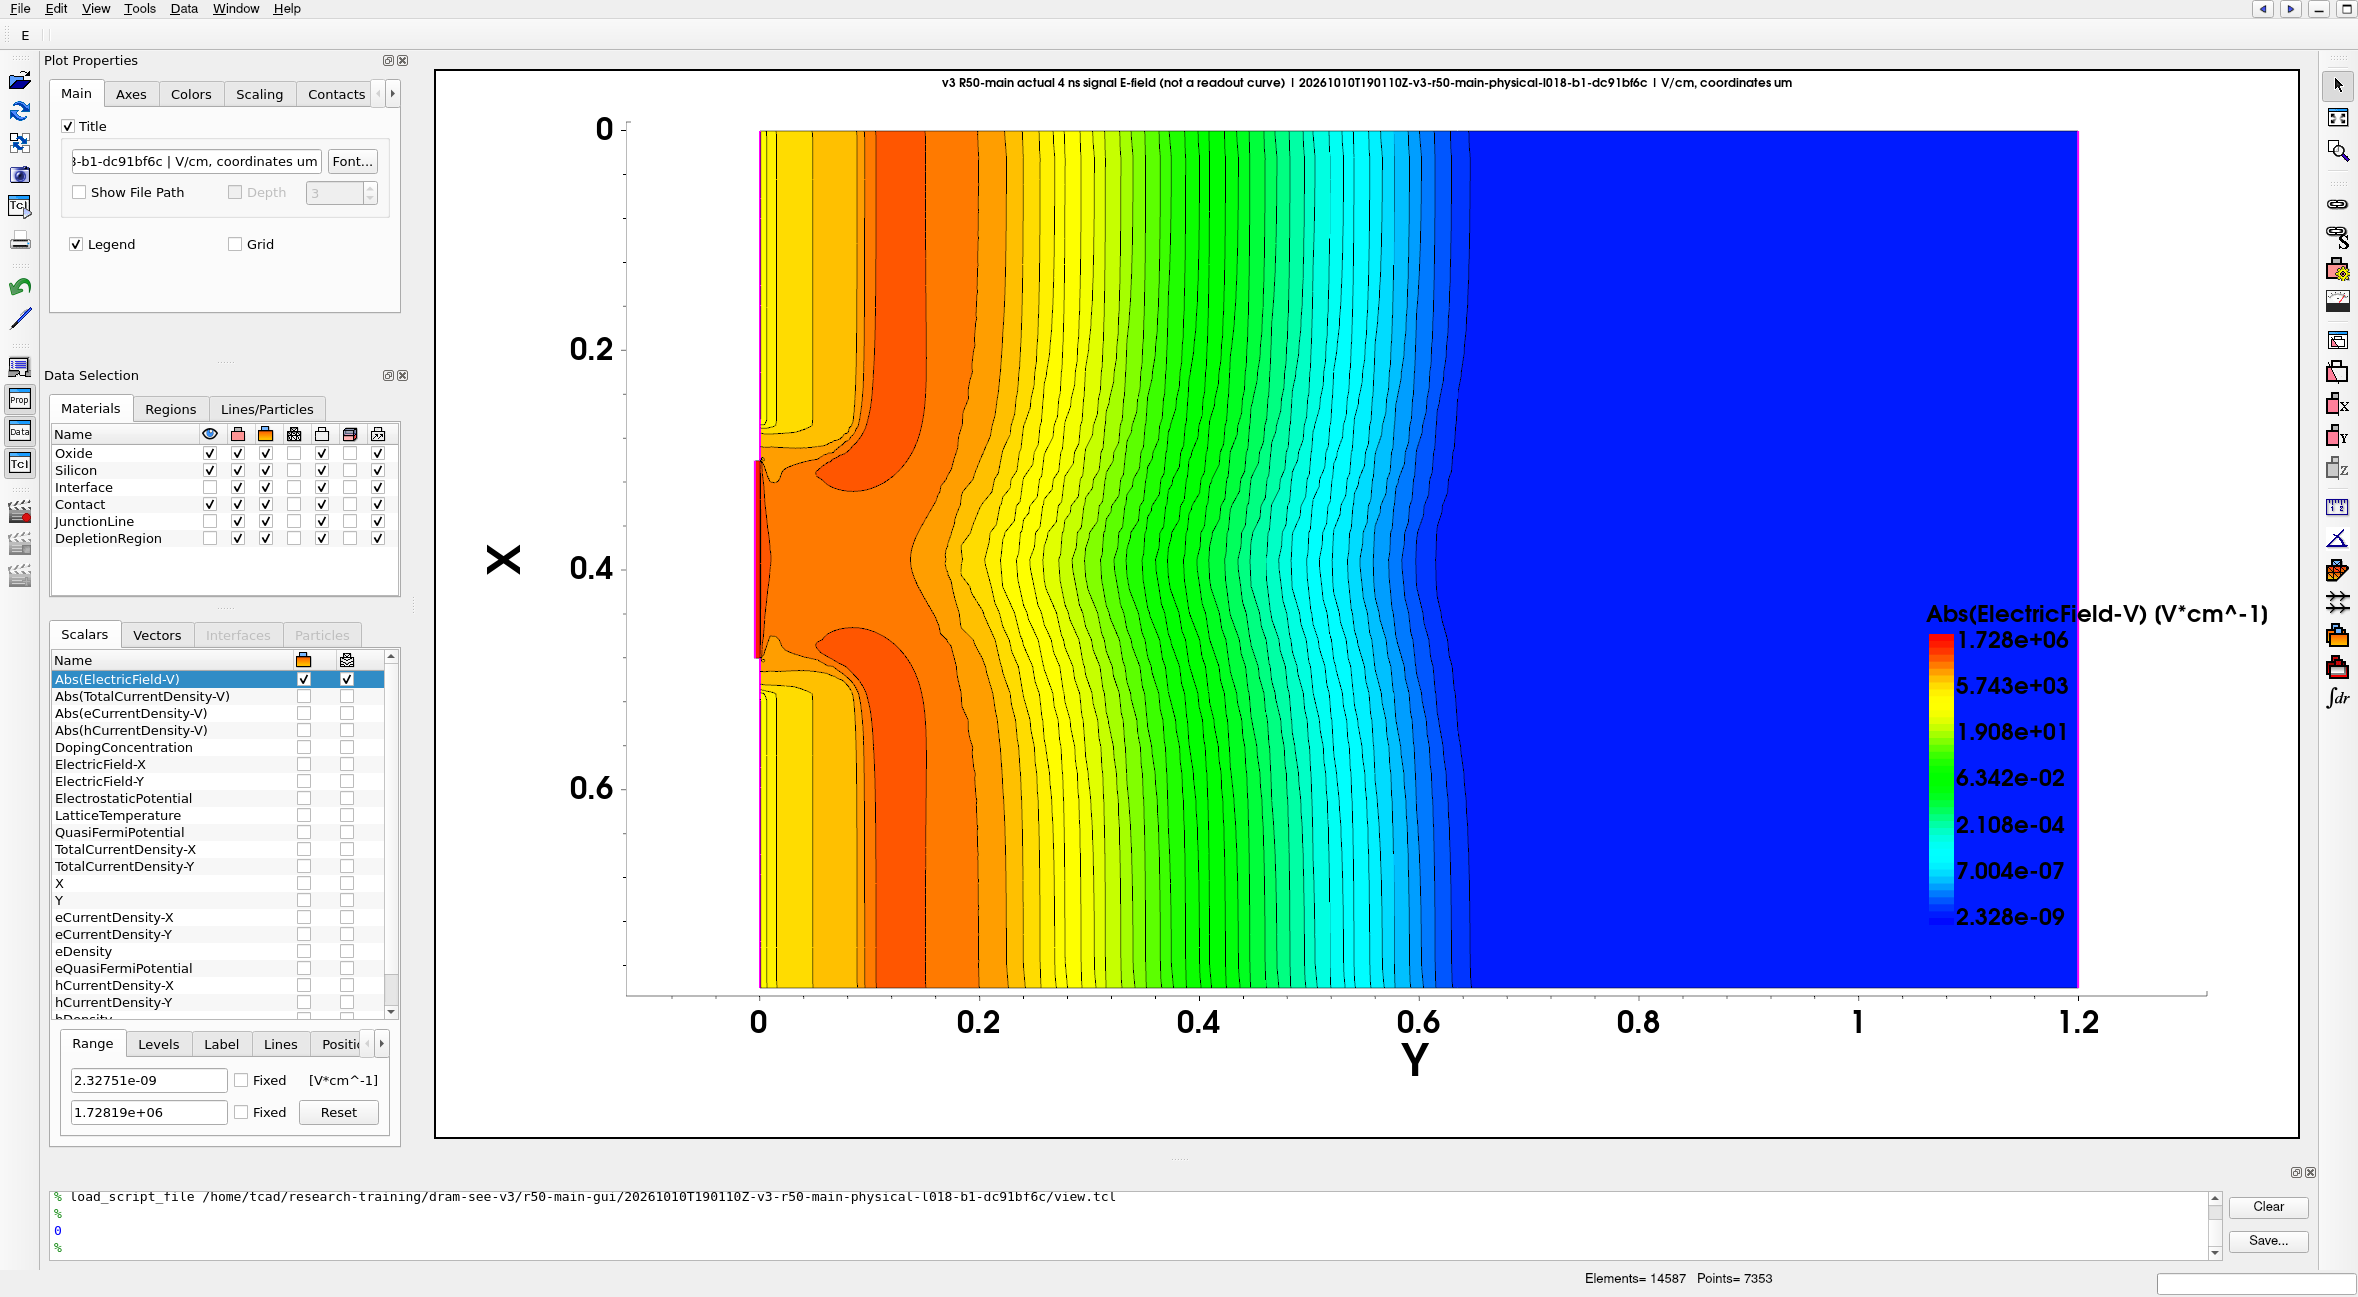
\includegraphics[width=.95\textwidth]{native-physical-window.png}
\caption{真实SVisual owned窗口：0.18~$\mu$m存储1物理参考，4~ns，Abs(ElectricField-V)，V/cm。完整窗口原字节保留并经主代理逐图目视。}
\label{cr:nativephysical}
\end{figure}

\begin{figure}[htbp]
\centering
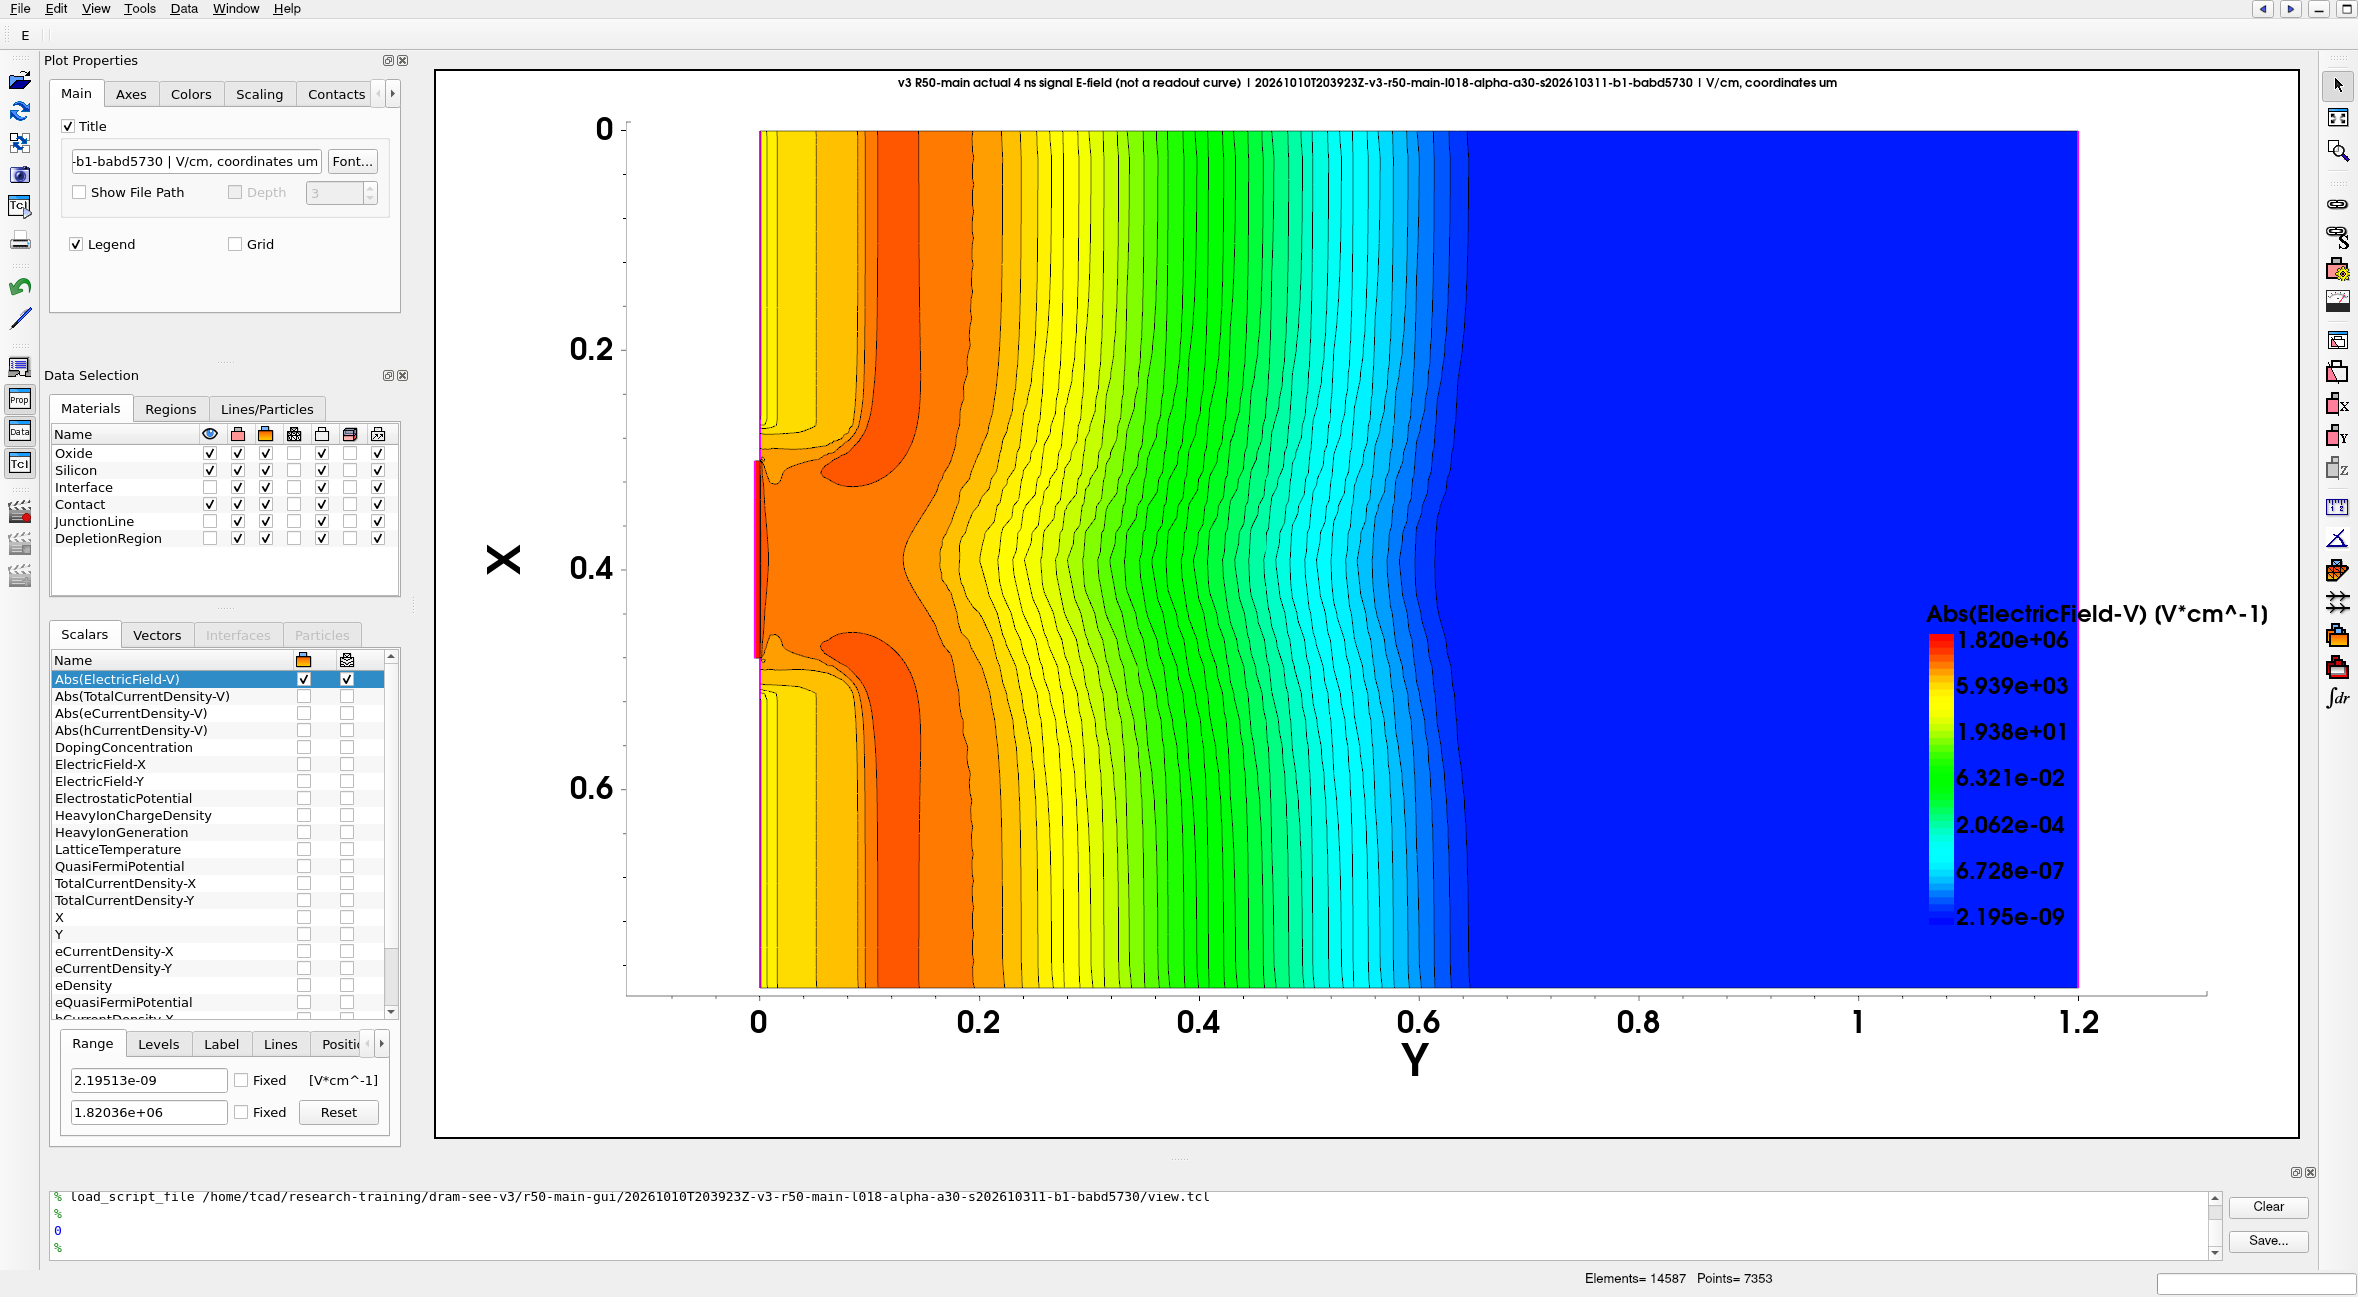
\includegraphics[width=.95\textwidth]{native-event-window.png}
\caption{真实SVisual owned窗口：0.18~$\mu$m、alpha、30°、seed202610311、bit1，4~ns。所示为原窗口，不是数据后处理绘图。}
\label{cr:nativeevent}
\end{figure}
对应1400×1000原生导出右端图例单位后缀存在裁切，已保留并如实记录；本文只展示同组完整owned窗口。真实窗口证明声明的run/变量/时刻，不证明通过Workbench Run按钮调度。
\subsection{失败保全与完整费用}

\begin{table}[htbp]
\centering\small
\caption{四个主线原始工程FAILED及其有效alias。null表示原始退出码未观测，不补写为0。}
\label{cr:failures}
\begin{tabular}{llll}
\toprule
原seed/位 & 有效重试版本 & 原状态 & 原runner退出码\\
\midrule
202610394-b1 & retry-r2 & FAILED & null（未观测）\\
202610353-b0 & retry-r3 & FAILED & null（未观测）\\
202610361-b0 & retry-r3 & FAILED & null（未观测）\\
202610371-b1 & retry-r4 & FAILED & null（未观测）\\
\bottomrule
\end{tabular}

\end{table}
完整历史账本共有7条FAILED记录；表中四项仅是R50主矩阵对应的确定性重试别名。最终逻辑槽失败为0，不表示历史失败为0，全部7条仍在原账本和快照中保留。
唯一全局账本已结算100022.07~s，约27.784~h；含原版本、probe、失败、重试与扩展。当前授权无上限，未结0项、费用缺项0项。该累计求解成本不是学生投入时长或AI效率对照。
\FloatBarrier

\section{失败解释、科学边界与AI使用}
\label{cr:discussion}
\subsection{工程恢复不会增加科学样本}
R50主线经历四次原始工程失败，其有效确定性重试分别由r2、r3和r4版本接续。
原始失败的退出码未被观测时仍保留为空值；后续收集成功或重试成功不能改写原始退出码。
四个alias只把真实通过的归档放回原逻辑槽，主分母仍是64个独立事件及128个配对响应。
正式统计不读取原FAILED的电学输出来选择更有利的结果，全部历史成本留在唯一账本。
原100~$\Omega$预充失败与独立probe另属历史阶段，也不加入R50主矩阵。

工程完成与科学有效性需分别判断。完整归档和退出0只能证明执行链满足工程条件；
初态、预充、积分、守恒、真实终点与匹配参考仍须通过科学审计。
旧100~$\Omega$预充误差超限时，即使最终裕量看似安全也不能纳入主线。
50~$\Omega$修订改变了外部电路，依靠新版本、新参考和新响应建立证据，原阈值没有放宽。

\subsection{连续量、读出判据与数值不确定性}
同方向的SN扰动对存储0与存储1可能有不同影响。
式\eqref{cr:metrics}用位值符号定义裕量，因而$\Delta M$可以为负，表示相对无粒子对照的裕量增加。
生成电荷、端口收集电荷和存储电容净变化不能互相替代；复合、不同端口收集及电容耦合共同作用。
因此不能以$Q_{\mathrm{dep}}/C$代替实际瞬态求解。

本次边界验证按完整128响应的预定距离排序选择两个目标，不以输出是否有利改变目标。
连续变化通过容差，不等于全部离散类别已确定。未选中但仍距某阈值不超过0.5~mV的响应，
若没有规定的两项匹配细化，仍按近界不确定处理。
原始分类与最终有效分类同时保留；临界和类别跨界不会自动抹去有限的连续目标，
连续数值失败则传播到有效评分标记。

每个位值/尺寸/粒子/方向分层只有四个独立事件。零次明确误读不能证明概率为零，
未知和临界状态需要用固定分母及最佳/最差包络解释。配对两位、工程重试和扩展不能把N翻倍。
本研究没有真实感放锁存、恢复与长期保持测试，固定4~ns采样的判据误读不能解释为持久位翻转。

\subsection{预测验证的含义}
模型先于测试TCAD提交冻结，测试仅用于评价固定预测。域内留出和尺寸外推分别给出
MAE、RMSE、最大绝对误差及基准比较，不将训练LOCO误差当作独立测试性能。
模型的输入包含真实Geant4沉积量，其用途是给定源项及基线条件后的TCAD响应近似，
并未替代全部输运或基准仿真。
本次完整测试评价扩大了已验证范围，但范围仍限于指定四栅长、两粒子、单一5~MeV能量和两个方向。
不能由固定集合表现推断任意粒子谱、入射位置或新工艺节点。

\subsection{受控初态、二维模型和材料栈限制}
存储0/1由理想钳位及准静态初态建立，随后释放钳位并检查粒子前电压。
这一设计控制初始条件，不能说明实际访问管能够在同样时间内写入，亦未校准写入能耗或保持可靠性。
二维平面器件、1~$\mu$m有效厚度、理想集总电容和固定掺杂均是探索设定。
数值一致性只能检验当前方程和离散实现，不能发现共同的模型系统偏差。

Geant4采用硅/真空几何与电磁option4。质子结果限于所用电磁配置的电离响应，
不能写为已经验证核反应次级粒子或核反冲主导的SEE。
4/6~nm氧化层结果使用同一硅入口事件，只是TCAD参数敏感性；未重算变化材料栈中的完整输运。
总量等效直径迹也没有保留完整三维逐步能量沉积的空间和时间分布。

\subsection{AI作用与课程责任}
AI协助文献组织、脚本开发、失败取证、证据核验、图表和文稿编写；固定代码承担参数映射、
求解顺序、阈值判断和评分。没有开展人工操作对照实验，不能报告AI加速倍数或因果效率优势。
工程流水线完成不说明学生已独立理解或操作；小组人数、真实贡献、教师审核、资源交接、
组内试讲、现场演示、答辩与成绩均保留待人工记录。
后续器件研究需要有出处的工艺结构和电学数据校准，课程验收则需要真实参与者完成相应教学活动。

\section{结论与后续工作}
在5~mV主阈值下，128个响应中96项正确、20项判据误读、8项临界、4项数值不确定，失败和缺失各为0与0项。域内留出的存储0/1岭回归RMSE分别为0.088294/0.094644~fC（电荷）和0.798415/0.838043~mV（裕量损失）。尺寸外推的存储0/1岭回归RMSE分别为0.068049/0.067155~fC（电荷）和0.519434/0.504929~mV（裕量损失）。
本次完成了限定自然语言映射、真实事件到器件源项传递、匹配参考定义、统一主矩阵、预测前冻结、独立留出/外推评分与受控扩展的一致证据链。原科学门槛、样本分母和全部失败保持不变。边界验证显示连续量稳定与分类稳定需要分别报告，不能以一次连续门槛通过清除全部数值不确定。

下一步器件研究需用具有出处的工艺和电学数据校准结构、实际写入、保持、感放及恢复，扩展能量、位置与统计规模。课程方面已形成可编辑报告、研究稿、PPT与只读演示材料；真实学生贡献、教师审核、试讲、答辩和考核由参与者完成并据实留证。

\FloatBarrier\clearpage
\bibliographystyle{unsrt}\bibliography{references}
\clearpage\appendix
\ctexset{section={name={附录,},number=\Alph{section}}}
\section{课程要求与代理可交付材料}
\small
\begin{longtable}{p{0.22\textwidth}p{0.43\textwidth}p{0.27\textwidth}}
\toprule 课程要求&本次可核查技术材料&待人工完成或适用限制\\\midrule
\endfirsthead\toprule 课程要求&本次可核查技术材料&待人工完成或适用限制\\\midrule\endhead
DRAM、SEE与AI方法&第1至4章、公式及参数来源&学生个人理解与答辩表现\\
2至3人合作&可按模型、平台、数据分析登记职责&姓名、学号、真实贡献和日期\\
可行性、方案、步骤和进度&第1、4、5章与materials索引&教师对方案和变更的审核\\
环境与资源&Windows和Linux VM的真实远程访问式流程&实验室服务器/模型正式交接\\
基础模型与源项传递&二维1T1C输入、G4事件、源积分审计&未校准真实DRAM工艺\\
自然语言参数遍历&R50已验收preview/audit/locate及拒绝行为&学生现场演示尚未发生\\
多尺寸/粒子/方向评估&完整64事件、128响应与固定分层&范围外的能量、位置与工艺未验证\\
拟合、外推与验证&训练LOCO、64冻结预测及全量独立评分&未建立商业可靠性外推\\
工艺与数值敏感性&14氧化层case、固定两边界目标及匹配细化&未完成变化材料栈的输运重算\\
总结与作品演示&完整报告、研究稿、PPT及只读演示脚本&教师评审、试讲、答辩、考核待发生\\
\bottomrule\end{longtable}\normalsize
\section{成员与实际活动登记}
指导教师李洋来自课程大纲，不能据此声称本报告已获教师审核。
真实参与者应填写成员姓名/学号、职责、完成时间与可核查贡献，并另存方案审核、
资源交接、试讲反馈、正式演示/答辩及教师考核记录。AI工具不计作小组成员。
课程评分权重为导师20\%、报告20\%、答辩或作品演示60\%；本报告不预测成绩。

\section{只读复现与演示}
\begin{enumerate}
\item 核验本包\sourcepath{sources.json}、\sourcepath{delivery-manifest.json}及输入快照清单，说明固定分母和模型边界。
\item 展示受约束R50请求的预览、审计与指定事件定位。历史映射快照的24小时语法字段不决定当前无限预算。
\item 选择一行\sourcepath{data/snapshot/response-sources.json}，定位actual tag、owner plan、case-freeze、run ID和input/archive SHA。
\item 对照源事件和匹配control/neutral，解释2.8~ns的$\Delta Q$及4~ns的$D,M,\Delta M$。
\item 展示预测冻结时间及真实测试提交索引，分别解释留出/外推误差、原r4评分和最终数值证据评分。
\item 展示DATA PLOT、原生场图和owned窗口的不同证据用途；核场变量、单位、4~ns和run来源。
\item 解释R50主线四个原始FAILED、null退出码及相应确定性重试；完整历史账本7条FAILED均保留，费用以完整唯一账本为准。
\end{enumerate}
上述是供参与者采用的步骤，不是已完成学生现场演示记录。耗时求解使用事先冻结归档并明确标注预先运行；
本报告构建及演示资料均不启动新仿真。
\par\medskip\noindent
\begin{tabular}{lp{0.62\textwidth}}
\toprule
证据类别 & 本包入口\\
\midrule
完整128槽及数值状态 & \sourcepath{data/snapshot/responses.csv}\\
真实case owner与四alias & \sourcepath{data/snapshot/response-sources.json}\\
原FAILED和费用 & \sourcepath{data/snapshot/ledger-snapshot.json}\\
原r4固定模型评分 & \sourcepath{data/snapshot/original-r4-prediction-scores.json}\\
最终数值证据评分 & \sourcepath{data/snapshot/final-numerical-prediction-scores.json}\\
原生PNG真实目视 & \sourcepath{data/native-visual-review.json}\\
全部来源与哈希 & \sourcepath{sources.json}\\
\bottomrule
\end{tabular}


\end{document}
